% ACS Environmental Science & Technology - Supporting Information
% Separate file submitted alongside main manuscript

\documentclass[journal=esthag,manuscript=suppinfo]{achemso}

\usepackage[version=4]{mhchem}
\usepackage{siunitx}
\usepackage{graphicx}
\usepackage{booktabs}
\usepackage{longtable}

\graphicspath{{Data/final-figs/}{Data/}}

% ============================================================================
% TITLE AND AUTHORS (must match main manuscript)
% ============================================================================

\author{Isaac N. Aguilar}
\affiliation{Division of Geological and Planetary Sciences, California Institute of Technology, Pasadena, California, 91125}
\email{iaguilar@caltech.edu}

\title{Supporting Information: Rapid detection of metal contamination in ash on outdoor surfaces after the 2025 Eaton Fire in a Wildland-Urban Interface}

\begin{document}

% ============================================================================
% TABLE OF CONTENTS FOR SI
% ============================================================================

\section*{Contents}

\begin{itemize}
  \item \S 1. Two-stage XRF calibration
  \begin{itemize}
    \item Kaolinite-clay calibration standard preparation protocol
    \item Table S1. PBP clay reference series
    \item Table S2. Stage A clay-calibration coefficients
    \item Figure S1. Clay calibration curves (4 arms)
    \item Table S3. Pb~L-line sweep results
  \end{itemize}
  \item \S 2. Alternative calibration approaches
  \begin{itemize}
    \item Table S4. Full 4-arm validation metrics
    \item Figure S2. XRF vs.\ ICP-MS validation (4 panels)
    \item Figure S3. Method-agreement ratio plots (4 panels)
    \item Table S5. Threshold classification (4 arms $\times$ 6 thresholds)
    \item Table S6. Cumulative classification summary
  \end{itemize}
  \item \S 3. Ash-matrix correction and outlier handling
  \begin{itemize}
    \item Table S7. Matrix-correction slopes
    \item Table S8. Outlier-handling sensitivity
  \end{itemize}
  \item \S 4. Sample metadata
  \begin{itemize}
    \item Table S9. Sample locations and collection metadata
    \item Machine-readable datasets (CSV) available at Zenodo
  \end{itemize}
\end{itemize}

\newpage

% ============================================================================
% S1. TWO-STAGE XRF CALIBRATION
% ============================================================================

\section*{S1. Two-stage XRF calibration: clay-pellet calibration and line selection}

\subsection*{Kaolinite-clay calibration standard preparation}

% TODO (author): replace this placeholder with the lab protocol for the
% PBP01--PBP04 standard synthesis. Suggested content: source of kaolinite
% (vendor and grade), Pb spike compound (e.g., Pb(NO$_3$)$_2$), gravimetric
% mixing procedure, drying conditions, sieve fraction used, certification
% workflow, and any QA/QC steps. The numerical Pb spike concentrations are
% summarized in Table S1.
\textit{[Insert author's lab protocol describing how the PBP01--PBP04
kaolinite-clay calibration standards were prepared, including: kaolinite
source and grade; Pb spike compound and addition procedure; gravimetric
mixing and drying steps; final sieve fraction; and QA/QC certification of
the nominal Pb concentrations.]}

\subsection*{Clay reference standards}

We used the PBP01--PBP04 clay reference series for instrument calibration. Each series is a kaolinite-based clay matrix doped with certified Pb concentrations of 100, 500, 1000, and 0~ppm respectively (PBP04 is the blank). Three replicate preparations were made per series for each preparation method (pellet pressing and loose powder), yielding 12 pellet and 12 powder calibration points; one powder replicate (PBP04\_powder\_1) returned no detectable Pb peak and was excluded, leaving $n=11$ for powder calibrations. Replicate-level standard deviations within a series are well below the inter-series differences, supporting the use of all replicates as independent calibration points.

\begin{table}[htbp]
\caption{PBP clay reference series.}
\label{tab:pbp_series}
\centering
\begin{tabular}{lrr}
\toprule
Series & Known Pb (ppm) & Replicates per prep method \\
\midrule
PBP01 & 100  & 3 \\
PBP02 & 500  & 3 \\
PBP03 & 1000 & 3 \\
PBP04 & 0 (blank) & 3 \\
\bottomrule
\end{tabular}
\end{table}

\subsection*{Stage A clay calibration: 4-arm performance}

For each preparation method, we fit a linear calibration of the form
$\widehat{\text{Pb}}_{\text{ppm}} = a + b \cdot \text{response}$
on the PBP standards. The fundamental-parameters (FP)-derived concentration was used as the response for the FP arms; the empirically selected line-intensity model (see Line Selection Sweep below) was used for the intensity arms. Pellet-intensity uses the multi-predictor Pb~L$\beta_1$+L$\beta_2$ model; powder-intensity uses Pb~L$\beta_1$+L$\beta_3$.

\begin{table}[htbp]
\caption{Stage A clay-calibration coefficients on PBP standards. LOOCV RMSE is the leave-one-out cross-validated prediction RMSE on the calibration set itself.}
\label{tab:stage_a_calibration}
\centering
\small
\begin{tabular}{llrrrr}
\toprule
Method & Response & $n$ & Cal $R^2$ & Cal RMSE (ppm) & LOOCV RMSE (ppm) \\
\midrule
pellet$_{\mathrm{intensity}}$  & Pb~L$\beta_1$ + L$\beta_2$ (multi)      & 12 & 0.999 & 14.4 & 19.5  \\
powder$_{\mathrm{intensity}}$  & Pb~L$\beta_1$ + L$\beta_3$ (multi)      & 11 & 0.937 & 97.9 & 361   \\
pellet$_{\mathrm{FP}}$         & FP-derived ppm                         & 12 & 0.995 & 27.6 & 32.7  \\
powder$_{\mathrm{FP}}$         & FP-derived ppm                         & 11 & 0.913 & 116  & 138   \\
\bottomrule
\end{tabular}
\end{table}

Stage A coefficients for all four arms are visualized in Figure~S1.

\begin{figure*}[htbp]
\centering

\includegraphics[width=\textwidth]{Fig_calibration_4panel.png}
\caption{Stage A clay calibration on PBP01--PBP04 reference standards. Each panel shows known Pb concentration (x-axis) vs.\ predicted Pb concentration (y-axis) under the indicated calibration arm. Solid blue lines are the fitted regressions; the four PBP series are color-coded. Pellet preparations (top row) are tighter than powder (bottom row); intensity-based responses (right column) outperform fundamental-parameters concentration for both prep methods.}
\label{fig:calibration_4panel}
\end{figure*}

\subsection*{Pb~L-line sweep: candidate calibration models built from the 6 deposited lines}

The Zenodo deposit contains six Pb~L-line intensities (L$\alpha_1$, L$\alpha_2$, L$\beta_1$, L$\beta_2$, L$\beta_3$, L$\beta_4$). For each preparation method (pellet, powder), we fit candidate calibration models built from these lines as single-line, sum, and multi-predictor responses, ran each through the full prediction pipeline (clay calibration, ash-matrix correction with Cook's $D$ filtering, validation against ICP-MS), and ranked candidates by validation RMSE (Table~\ref{tab:line_sweep}). The a~priori interference assessment for context:

\begin{table}[htbp]
\caption{A priori spectral interference assessment for Pb L-lines in the ash matrix. As, Rb, Sr, and Y were detected in the ICP-MS reference data at concentrations sufficient to produce overlapping K-shell emission in XRF.}
\label{tab:line_interferences}
\centering
\small
\begin{tabular}{lll}
\toprule
Pb line (energy, keV) & Overlapping element line & Decision \\
\midrule
L$\alpha_1$ (10.55) & As K$\alpha$ (10.54)            & swept (As Kα interference) \\
L$\alpha_2$ (10.45) & As K$\alpha$ (10.54)            & swept (As Kα interference) \\
L$\beta_1$ (12.61)  & clear region                    & swept \\
L$\beta_2$ (12.62)  & clear region                    & swept \\
L$\beta_3$ (12.79)  & Th L$\alpha$ (12.97) -- minor  & swept \\
L$\beta_4$ (12.31)  & clear region                    & swept \\
\bottomrule
\end{tabular}
\end{table}

For each prep method, twelve candidate response variables were tested: six single-line responses (L$\alpha_1$, L$\alpha_2$, L$\beta_1$, L$\beta_2$, L$\beta_3$, L$\beta_4$), four sum responses (L$\alpha_1$+L$\alpha_2$, L$\beta_1$+L$\beta_2$, L$\beta_1$+L$\beta_3$, L$\beta_1$+L$\beta_2$+L$\beta_3$+L$\beta_4$), and two multi-predictor responses (L$\beta_1$,L$\beta_2$ and L$\beta_1$,L$\beta_3$). Candidates were ranked by validation RMSE against ICP-MS rather than calibration $R^2$, and the best response per prep method was carried into the headline 4-arm validation in the main text. The complete 24-row sweep is in \texttt{Table\_S3\_pb\_line\_sweep.csv}; the top entries per method are summarized below.

\begin{table}[htbp]
\caption{Top candidate Pb~L-line response variables per preparation method, ranked by validation RMSE against ICP-MS through the full two-stage pipeline. The L$\beta_1$,L$\beta_2$ multi-predictor wins for pellet; the L$\beta_1$,L$\beta_3$ multi-predictor wins for powder. Single-line and sum responses are 4--7$\times$ worse on validation RMSE for pellet, and the L$\beta_1$,L$\beta_2$ multi-predictor collapses on powder, motivating the per-arm choice of multi-predictor composition.}
\label{tab:line_sweep}
\centering
\small
\begin{tabular}{llrrrrrr}
\toprule
Method & Response & $n_{\mathrm{val}}$ & Cal $R^2$ & Val $r$ & Val RMSE & BA bias & BA LOA range \\
       &          &                     &           &          & (ppm)    & (ppm)   & (ppm)        \\
\midrule
pellet & \textbf{Pb~L$\beta_1$, L$\beta_2$ (multi)} & 33 & 0.999 & 0.999 &  151 &  $-2$  &   601 \\
pellet & Pb~L$\alpha_1$ (single)                    & 33 & 0.998 & 0.998 &  719 & $+125$ & 2819 \\
pellet & Pb~L$\alpha_2$ (single)                    & 32 & 0.998 & 0.998 &  726 & $+127$ & 2846 \\
pellet & Pb~L$\alpha_1$+L$\alpha_2$ (sum)           & 32 & 0.998 & 0.998 &  730 & $+128$ & 2862 \\
pellet & Pb~L$\beta_1$, L$\beta_3$ (multi)          & 33 & 0.998 & 0.998 &  787 & $+142$ & 3084 \\
pellet & Pb~L$\beta_4$ (single)                     & 33 & 0.998 & 0.998 &  789 & $+139$ & 3090 \\
\midrule
powder & \textbf{Pb~L$\beta_1$, L$\beta_3$ (multi)} & 33 & 0.937 & 0.998 &  282 &  $+36$ &  1114 \\
powder & Pb~L$\alpha_2$ (single)                    & 32 & 0.904 & 0.990 & 1633 & $+308$ &  6387 \\
powder & Pb~L$\beta_4$ (single)                     & 33 & 0.904 & 0.989 & 1671 & $+311$ &  6537 \\
powder & Pb~L$\beta_2$ (single)                     & 33 & 0.904 & 0.989 & 1676 & $+311$ &  6556 \\
powder & Pb~L$\beta_1$+L$\beta_2$ (sum)             & 33 & 0.904 & 0.989 & 1679 & $+312$ &  6569 \\
powder & Pb~L$\beta_1$, L$\beta_2$ (multi)          & 33 & 0.928 & 0.913 & 2572 & $+471$ & 10067 \\
\bottomrule
\end{tabular}
\end{table}

The headline validation in the main text (Table~3) carries forward the best response for the recommended screening approach: \textbf{pellet$_{\mathrm{intensity}}$ = Pb~L$\beta_1$, L$\beta_2$ (multi)}. Notably the pellet- and powder-best multi-predictor compositions are not interchangeable: the L$\beta_1$,L$\beta_2$ pair that wins for pellet has the worst validation RMSE for powder (2{,}572~ppm vs.\ 282~ppm for L$\beta_1$,L$\beta_3$), reflecting that grain-size and density variability of unpressed powder couples differently to adjacent Pb~L$\beta$ peaks than to the more separated L$\beta_1$/L$\beta_3$ pair.

\newpage

% ============================================================================
% S2. ALTERNATIVE CALIBRATION APPROACHES AND VALIDATION
% ============================================================================

\section*{S2. Alternative calibration approaches and validation}

This section provides full validation metrics for all four calibration approaches (pellet/powder $\times$ intensity/FP) for readers interested in technical comparison. The main text reports only the recommended pellet L$\beta_1$+L$\beta_2$ intensity model.

\subsection*{Full 4-arm validation against ICP-MS}

\begin{table}[htbp]
\caption{Validation of all four calibration arms against ICP-MS, after the two-stage clay calibration (Stage A; \S 1) and ash-matrix correction (Stage B; \S 3). All metrics are computed on the 33 fully paired ash samples with leave-one-out cross-validation of the matrix-correction slope; predicted concentrations from the clay-calibration extrapolation below the PBP01 (100~ppm) anchor are floor-clipped at 0 to retain the full paired set in every arm.}
\label{tab:s4_full_validation}
\centering
\small
\begin{tabular}{lrrrrrrr}
\toprule
Method & $n$ & $r$ & RMSE & MAE & BA bias & BA LOA & LOA range \\
    &     &     & (ppm) & (ppm) & (ppm) & (ppm) & (ppm) \\
\midrule
pellet$_{\mathrm{intensity}}$  & 33 & 0.999 &  151 &  64 & $-2$   & $[-302, +299]$   &  601 \\
powder$_{\mathrm{intensity}}$  & 33 & 0.998 &  282 & 117 & $+36$  & $[-521, +593]$   & 1114 \\
pellet$_{\mathrm{FP}}$         & 33 & 0.990 & 1726 & 363 & $+308$ & $[-3072, +3689]$ & 6760 \\
powder$_{\mathrm{FP}}$         & 33 & 0.983 & 1880 & 394 & $+319$ & $[-3370, +4007]$ & 7377 \\
\bottomrule
\end{tabular}
\end{table}

The pellet-intensity arm achieves 10$\times$ narrower Bland-Altman limits of agreement than the fundamental-parameters (FP) approaches, despite all four arms showing high Pearson correlation ($r > 0.98$). The FP arms exhibit systematic positive bias (+308 to +319~ppm) reflecting the instrument's matrix correction assumptions, which are calibrated for homogeneous geological samples rather than heterogeneous wildfire ash.

\begin{figure*}[htbp]
\centering
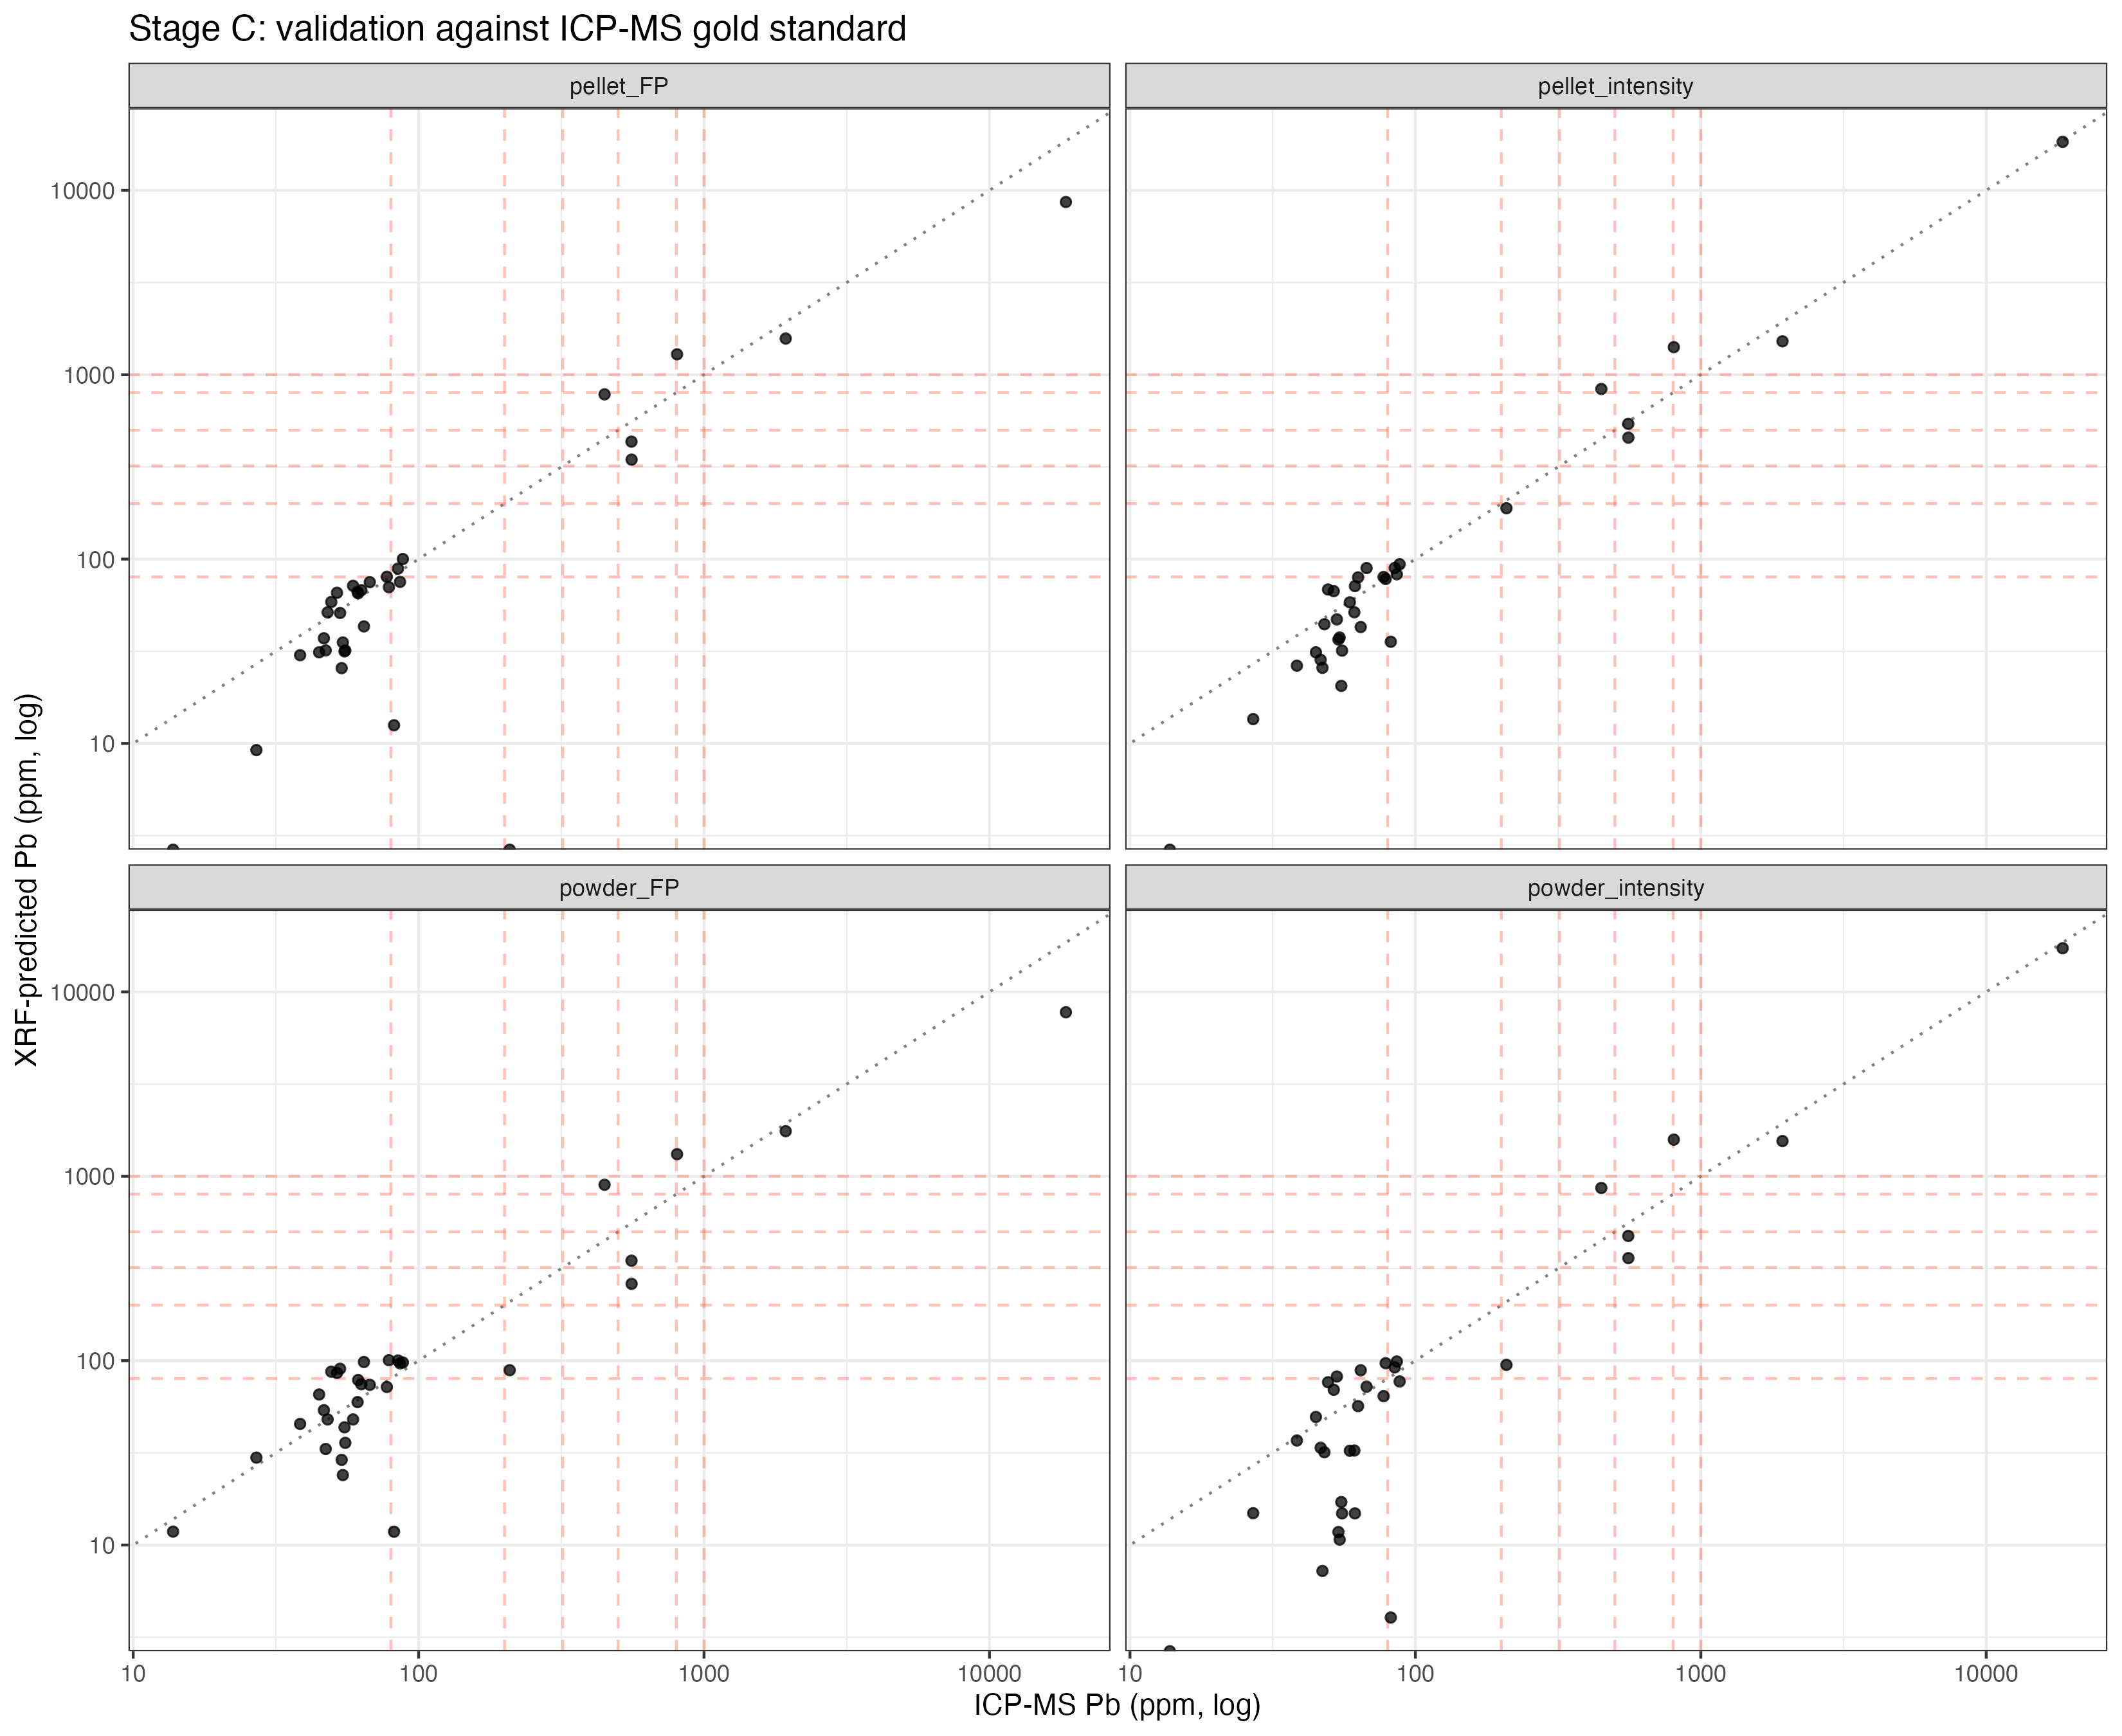
\includegraphics[width=\textwidth]{Fig_validation_4panel.png}
\caption{XRF-predicted Pb concentration vs.\ ICP-MS measured Pb (log-log scale) for the four calibration arms (panels ordered best-to-worst). Pellet preparations are coloured purple; powder preparations orange. Dotted grey diagonal is the 1:1 line.}
\label{fig:s2_validation_4panel}
\end{figure*}

\begin{figure*}[htbp]
\centering
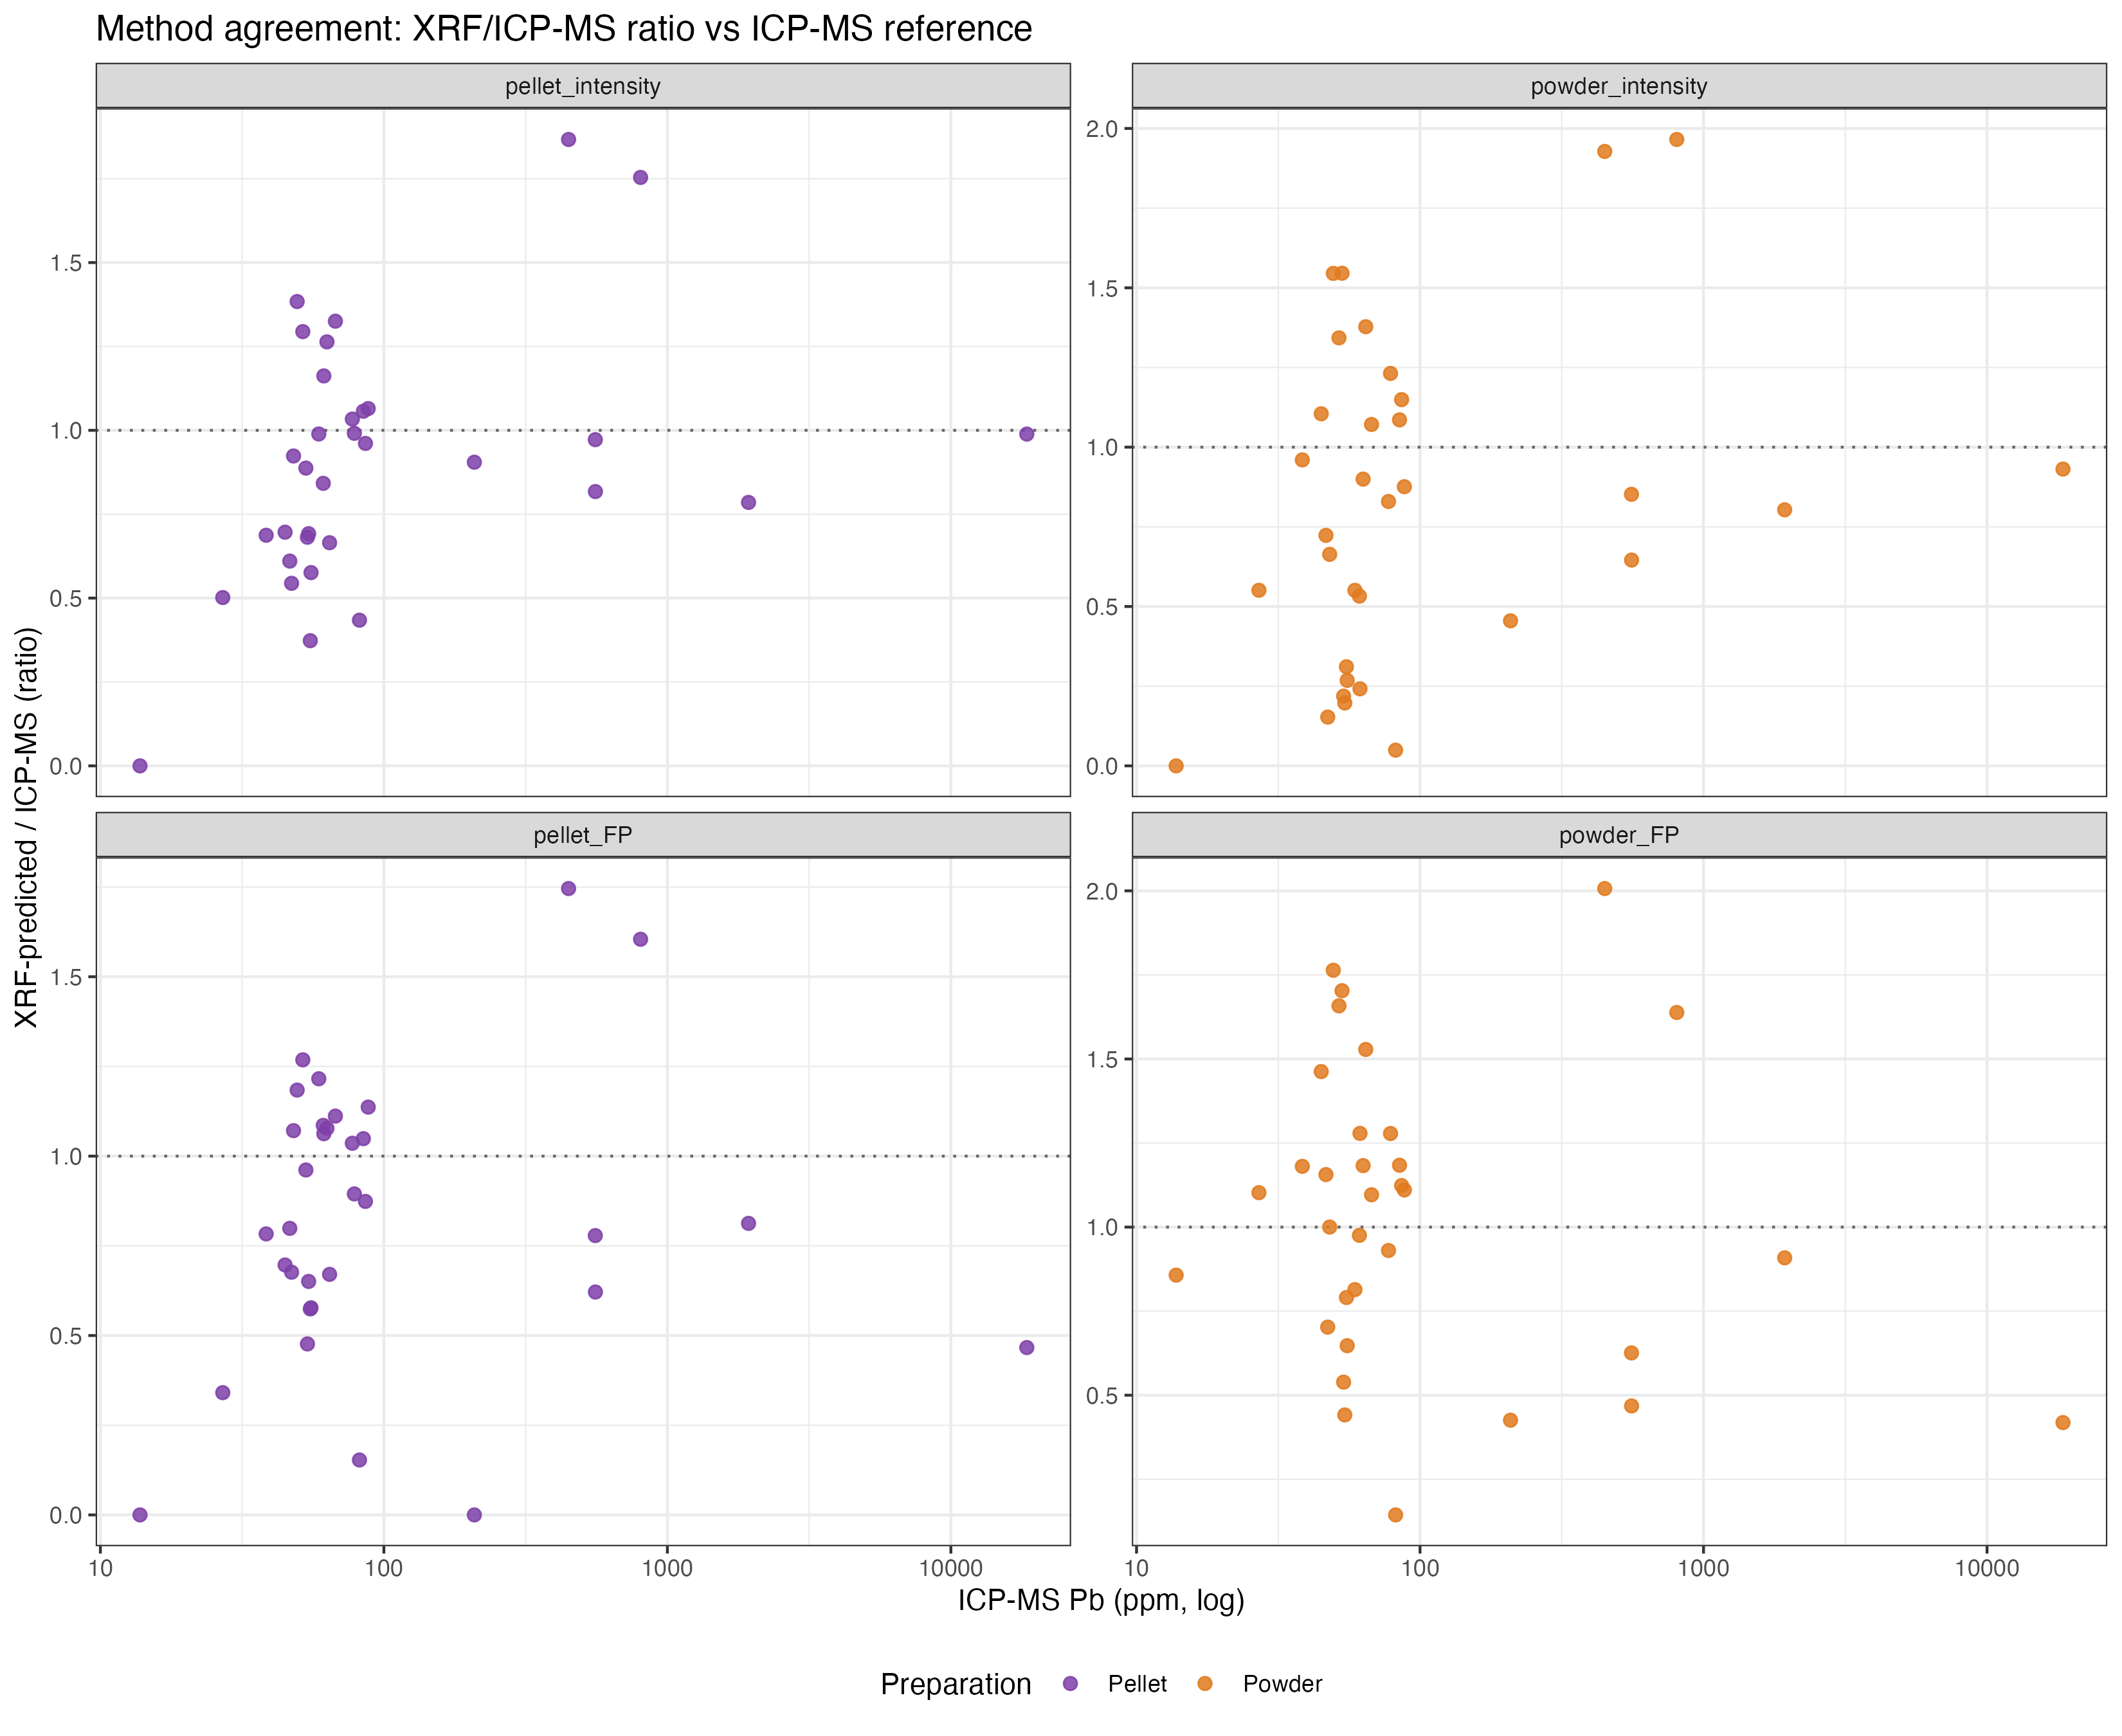
\includegraphics[width=\textwidth]{Fig_AgreementRatio_4panel.png}
\caption{Method-agreement ratio plots: XRF-predicted Pb divided by ICP-MS Pb (linear y-axis) versus ICP-MS Pb (log~x-axis) for the four calibration arms. The dotted grey reference line at ratio = 1 marks perfect agreement; values $<$1 indicate XRF under-prediction and $>$1 over-prediction. The pellet-intensity arm clusters tightly around 1.0 across the calibration range; the FP arms exhibit large ratio departures, especially for low-Pb samples.}
\label{fig:s3_ratio_4panel}
\end{figure*}

\subsection*{Full threshold classification (4 arms $\times$ 6 thresholds)}

\begin{table}[htbp]
\caption{Threshold classification performance on the 33 fully paired ash samples. For each Pb regulatory threshold and calibration arm we report the confusion matrix (TP, FN, FP, TN) and the Wilson 95\% binomial confidence intervals on sensitivity and specificity. Of the 33 paired samples, 11, 7, 6, 5, 3, and 2 exceeded the 80, 200, 320, 500, 800, and 1000~ppm thresholds, respectively.}
\label{tab:s5_threshold_classification}
\centering
\footnotesize
\begin{tabular}{l l c c c c c c c}
\toprule
Threshold & Method & TP & FN & FP & TN & Sensitivity (95\% CI) & Specificity (95\% CI) & Acc \\
(ppm)     &        &    &    &    &    &                       &                       &     \\
\midrule
\multirow{4}{*}{80}   & pellet$_{\mathrm{intensity}}$ & 10 & 1 & 1 & 21 & 0.91 [0.62, 0.98] & 0.95 [0.78, 0.99] & 0.94 \\
                      & powder$_{\mathrm{intensity}}$ & 9  & 2 & 3 & 19 & 0.82 [0.52, 0.95] & 0.86 [0.67, 0.95] & 0.85 \\
                      & pellet$_{\mathrm{FP}}$        & 8  & 3 & 1 & 21 & 0.73 [0.43, 0.90] & 0.95 [0.78, 0.99] & 0.88 \\
                      & powder$_{\mathrm{FP}}$        & 10 & 1 & 5 & 17 & 0.91 [0.62, 0.98] & 0.77 [0.57, 0.90] & 0.82 \\
\midrule
\multirow{4}{*}{200}  & pellet$_{\mathrm{intensity}}$ & 6 & 1 & 0 & 26 & 0.86 [0.49, 0.97] & 1.00 [0.87, 1.00] & 0.97 \\
                      & powder$_{\mathrm{intensity}}$ & 6 & 1 & 0 & 26 & 0.86 [0.49, 0.97] & 1.00 [0.87, 1.00] & 0.97 \\
                      & pellet$_{\mathrm{FP}}$        & 6 & 1 & 0 & 26 & 0.86 [0.49, 0.97] & 1.00 [0.87, 1.00] & 0.97 \\
                      & powder$_{\mathrm{FP}}$        & 6 & 1 & 0 & 26 & 0.86 [0.49, 0.97] & 1.00 [0.87, 1.00] & 0.97 \\
\midrule
\multirow{4}{*}{320}  & pellet$_{\mathrm{intensity}}$ & 6 & 0 & 0 & 27 & 1.00 [0.61, 1.00] & 1.00 [0.88, 1.00] & 1.00 \\
                      & powder$_{\mathrm{intensity}}$ & 6 & 0 & 0 & 27 & 1.00 [0.61, 1.00] & 1.00 [0.88, 1.00] & 1.00 \\
                      & pellet$_{\mathrm{FP}}$        & 6 & 0 & 0 & 27 & 1.00 [0.61, 1.00] & 1.00 [0.88, 1.00] & 1.00 \\
                      & powder$_{\mathrm{FP}}$        & 5 & 1 & 0 & 27 & 0.83 [0.44, 0.97] & 1.00 [0.88, 1.00] & 0.97 \\
\midrule
\multirow{4}{*}{500}  & pellet$_{\mathrm{intensity}}$ & 4 & 1 & 1 & 27 & 0.80 [0.38, 0.96] & 0.96 [0.82, 0.99] & 0.94 \\
                      & powder$_{\mathrm{intensity}}$ & 3 & 2 & 1 & 27 & 0.60 [0.23, 0.88] & 0.96 [0.82, 0.99] & 0.91 \\
                      & pellet$_{\mathrm{FP}}$        & 3 & 2 & 1 & 27 & 0.60 [0.23, 0.88] & 0.96 [0.82, 0.99] & 0.91 \\
                      & powder$_{\mathrm{FP}}$        & 3 & 2 & 1 & 27 & 0.60 [0.23, 0.88] & 0.96 [0.82, 0.99] & 0.91 \\
\midrule
\multirow{4}{*}{800}  & pellet$_{\mathrm{intensity}}$ & 3 & 0 & 1 & 29 & 1.00 [0.44, 1.00] & 0.97 [0.83, 0.99] & 0.97 \\
                      & powder$_{\mathrm{intensity}}$ & 3 & 0 & 1 & 29 & 1.00 [0.44, 1.00] & 0.97 [0.83, 0.99] & 0.97 \\
                      & pellet$_{\mathrm{FP}}$        & 3 & 0 & 0 & 30 & 1.00 [0.44, 1.00] & 1.00 [0.89, 1.00] & 1.00 \\
                      & powder$_{\mathrm{FP}}$        & 3 & 0 & 1 & 29 & 1.00 [0.44, 1.00] & 0.97 [0.83, 0.99] & 0.97 \\
\midrule
\multirow{4}{*}{1000} & pellet$_{\mathrm{intensity}}$ & 2 & 0 & 1 & 30 & 1.00 [0.34, 1.00] & 0.97 [0.84, 0.99] & 0.97 \\
                      & powder$_{\mathrm{intensity}}$ & 2 & 0 & 1 & 30 & 1.00 [0.34, 1.00] & 0.97 [0.84, 0.99] & 0.97 \\
                      & pellet$_{\mathrm{FP}}$        & 2 & 0 & 1 & 30 & 1.00 [0.34, 1.00] & 0.97 [0.84, 0.99] & 0.97 \\
                      & powder$_{\mathrm{FP}}$        & 2 & 0 & 1 & 30 & 1.00 [0.34, 1.00] & 0.97 [0.84, 0.99] & 0.97 \\
\bottomrule
\end{tabular}
\end{table}

\subsection*{Cumulative classification performance across methods}

\begin{table}[htbp]
\caption{Cumulative classification performance of the four calibration arms across the full regulatory range (six Pb thresholds: 80, 200, 320, 500, 800, and 1000~ppm). For each arm, the confusion matrix is pooled over all 33~samples~$\times$~6~thresholds = 198 binary-classification tests, with sample-level positive count $n_+ = 34$ (pooled across thresholds) and negative count $n_- = 164$. Wilson 95\% confidence intervals on sensitivity and specificity reflect the larger pooled denominators.}
\label{tab:s6_method_summary}
\centering
\small
\begin{tabular}{l c c c c c c c}
\toprule
Method & TP & FN & FP & TN & Sensitivity (95\% CI) & Specificity (95\% CI) & Acc \\
\midrule
pellet$_{\mathrm{intensity}}$  & 31 & 3 & 4 & 160 & 0.91 [0.77, 0.97] & 0.98 [0.94, 0.99] & 0.96 \\
powder$_{\mathrm{intensity}}$  & 29 & 5 & 6 & 158 & 0.85 [0.70, 0.94] & 0.96 [0.92, 0.98] & 0.94 \\
pellet$_{\mathrm{FP}}$         & 28 & 6 & 3 & 161 & 0.82 [0.67, 0.92] & 0.98 [0.95, 0.99] & 0.95 \\
powder$_{\mathrm{FP}}$         & 29 & 5 & 8 & 156 & 0.85 [0.70, 0.94] & 0.95 [0.91, 0.98] & 0.93 \\
\bottomrule
\end{tabular}
\end{table}

The pellet-intensity arm has the highest pooled sensitivity (0.91) and the lowest false-negative count (3 of 34), making it the recommended primary screening tool. The powder-intensity arm is the best field-portable alternative, with 0.85 pooled sensitivity and comparable specificity (0.96). The FP arms have lower cumulative sensitivity despite high specificity, reflecting the systematic positive bias that inflates predicted values and causes false negatives at lower thresholds.

\newpage

% ============================================================================
% S3. ASH-MATRIX CORRECTION AND OUTLIER HANDLING
% ============================================================================

\section*{S3. Ash-matrix correction and outlier handling}

\subsection*{Matrix-correction slopes (Stage B)}

For each calibration arm we fit a proportional regression
$\widehat{\text{Pb}}_{\text{ICP-MS}} = m_{\text{arm}} \cdot \widehat{\text{Pb}}_{\text{clay-pred}}$
on paired ash samples eligible for inclusion (i.e., excluding samples flagged by Cook's $D > 4/n$). The slope $m_{\text{arm}}$ absorbs the systematic clay-to-ash transfer bias arising from differing mass-attenuation coefficients of the two matrices.

\begin{table}[htbp]
\caption{Ash-matrix correction slopes and LOOCV stability. Eligible samples are those passing the Cook's $D > 4/n$ filter; excluded samples are still predicted (using the eligible-set full-fit slope) and contribute to the validation summary in main-text Table~3.}
\label{tab:s7_matrix_correction}
\centering
\small
\begin{tabular}{lrrrrr}
\toprule
Method & $n$ eligible & $n$ excluded & Excluded samples & Full-fit slope & LOOCV slope SD \\
\midrule
pellet$_{\mathrm{intensity}}$  & 31 & 2 & XPAH28, JPL73         & 2.723 & 0.092 \\
powder$_{\mathrm{intensity}}$  & 31 & 2 & XPAH28, JPL73         & 0.705 & 0.021 \\
pellet$_{\mathrm{FP}}$         & 30 & 3 & XPAH28, JPL73, XPAH20 & 1.144 & 0.056 \\
powder$_{\mathrm{FP}}$         & 30 & 3 & XPAH28, JPL73, XPAH20 & 0.334 & 0.023 \\
\bottomrule
\end{tabular}
\end{table}

Sample XPAH28 (ICP-MS Pb = 18,528~ppm) had extreme leverage in the proportional regression and was excluded from slope fitting in all arms; JPL73 (804~ppm) was also flagged. Excluded samples were still predicted using the eligible-set slope and contribute to validation metrics.

\subsection*{Outlier-handling sensitivity}

We compared three approaches for managing high-leverage samples: no exclusion, concentration-based exclusion, and Cook's distance--based exclusion. Cook's $D > 4/n$ filtering yielded the lowest validation RMSE and tightest agreement intervals (Table~\ref{tab:s8_outlier_sensitivity}).

\begin{table}[htbp]
\caption{Outlier-handling sensitivity for the pellet-intensity arm. All strategies validated on the complete 33-sample set; only the slope-fitting subset varied.}
\label{tab:s8_outlier_sensitivity}
\centering
\small
\begin{tabular}{lrrrr}
\toprule
Strategy & $n$ training & Val RMSE (ppm) & BA bias (ppm) & LOA range (ppm) \\
\midrule
All samples (no exclusion)        & 33 & 478  & $+59$  & 1890 \\
Drop highest sample (XPAH28)      & 32 & 492  & $+93$  & 1925 \\
\textbf{Cook's $D > 4/n$ (used)}  & \textbf{31} & \textbf{151} & \textbf{$-2$} & \textbf{601} \\
\bottomrule
\end{tabular}
\end{table}

\newpage

% ============================================================================
% S4. SAMPLE METADATA (renumbered from S5)
% ============================================================================

\section*{S4. Sample metadata}

\begin{table}[htbp]
\caption{Sample locations and collection metadata (excerpt; complete metadata in \texttt{sample\_id\_harmonization.csv}).}
\label{tab:s9_metadata}
\centering
\small
\begin{tabular}{lrrll}
\toprule
Sample ID & Latitude & Longitude & Collection Date & Sample Type \\
\midrule
1590  & 34.1399 & -118.0888 & 2025-01-15 & Ash \\
1620  & 34.1719 & -118.1235 & 2025-01-15 & Ash \\
GPS03 & 34.1300 & -118.1440 & 2025-01-16 & Ash \\
% ... additional rows ...
\bottomrule
\end{tabular}
\end{table}

\textit{Note.} Complete ICP-MS, XRF (cleaned and per-line intensities), PBP calibration, and validation paired datasets are provided as separate machine-readable CSV files. The full prediction pipeline — sample data cleaning, two-stage calibration, ash-matrix correction, validation, and figure/table generation — is reproducible from \texttt{D2D/XRF/scripts/eaton\_xrf\_pipeline.R}.

\end{document}
